\section{Reconocimiento facial invariante a la edad}

\subsection{Objetivos}
\begin{frame}{Objetivos}

	\begin{itemize}
		\item Resolver una tarea de \textbf{reconocimiento facial invariante a cambios en la edad}, por sus siglas en inglés, \textit{AIFR}.
		\item Estudiar dos variantes \textit{online} en la función de pérdida \textit{Triplet Loss}.
	\end{itemize}

\end{frame}

\subsection{Tarea a resolver}

\begin{frame}{\textit{AIFR}}

	\begin{figure}
		\includegraphics[width=0.8\textwidth]{informatica/ejemplo_dificultad_aifr}
		\caption{Ejemplo de datos con los que trabajamos en una tarea de \textit{AIFR}. Imagen extraída de \cite{informatica:aifr_survey}.}
		\label{img:ejemplo_dificultad_aifr}
	\end{figure}

\end{frame}

\begin{frame}{Problemas asociados a la tarea}

	\begin{itemize}
		\item Pueden ser más similares dos personas distintas de la misma edad que la misma persona en dos edades muy distantes.
		\item El envejecimiento modifica las características faciales.
		\item Trabajar con identidades nunca vistas.
		\item Escasez de conjuntos de datos para estudiar la tarea de \textit{AIFR}, que además presentan diversas dificultades.
	\end{itemize}

\end{frame}

\begin{frame}{Tarea concreta a resolver}

	Tarea de \textbf{verificación}:

	\begin{figure}[!h]
		\includegraphics[width=0.7\textwidth]{informatica/ejemplos_tareas/verification}
		\caption{Imágenes extraídas de \cite{informatica:cacd_dataset}.}
	\end{figure}


\end{frame}

\begin{frame}{\textit{AIFR}}

	Tarea de \textbf{\textit{retrieval}} o búsqueda:

	\begin{figure}[!h]
		\includegraphics[width=0.8\textwidth]{informatica/ejemplos_tareas/retrieval}
		\caption{Imágenes extraídas de \cite{informatica:cacd_dataset}.}
	\end{figure}

	Esta es la tarea en la que centramos nuestro estudio.

\end{frame}

\subsection{Enfoque}
\begin{frame}{Embedding semántico}

	\begin{itemize}
		\item Queremos que nuestra red aprenda un \textbf{\textit{embedding} semántico}.
		\item Elementos de la misma identidad deberán estar cerca entre sí, mientras que elementos de distintas identidades deberán estar distantes.
	\end{itemize}

\end{frame}

\begin{frame}{Embedding semántico}

	\begin{figure}
		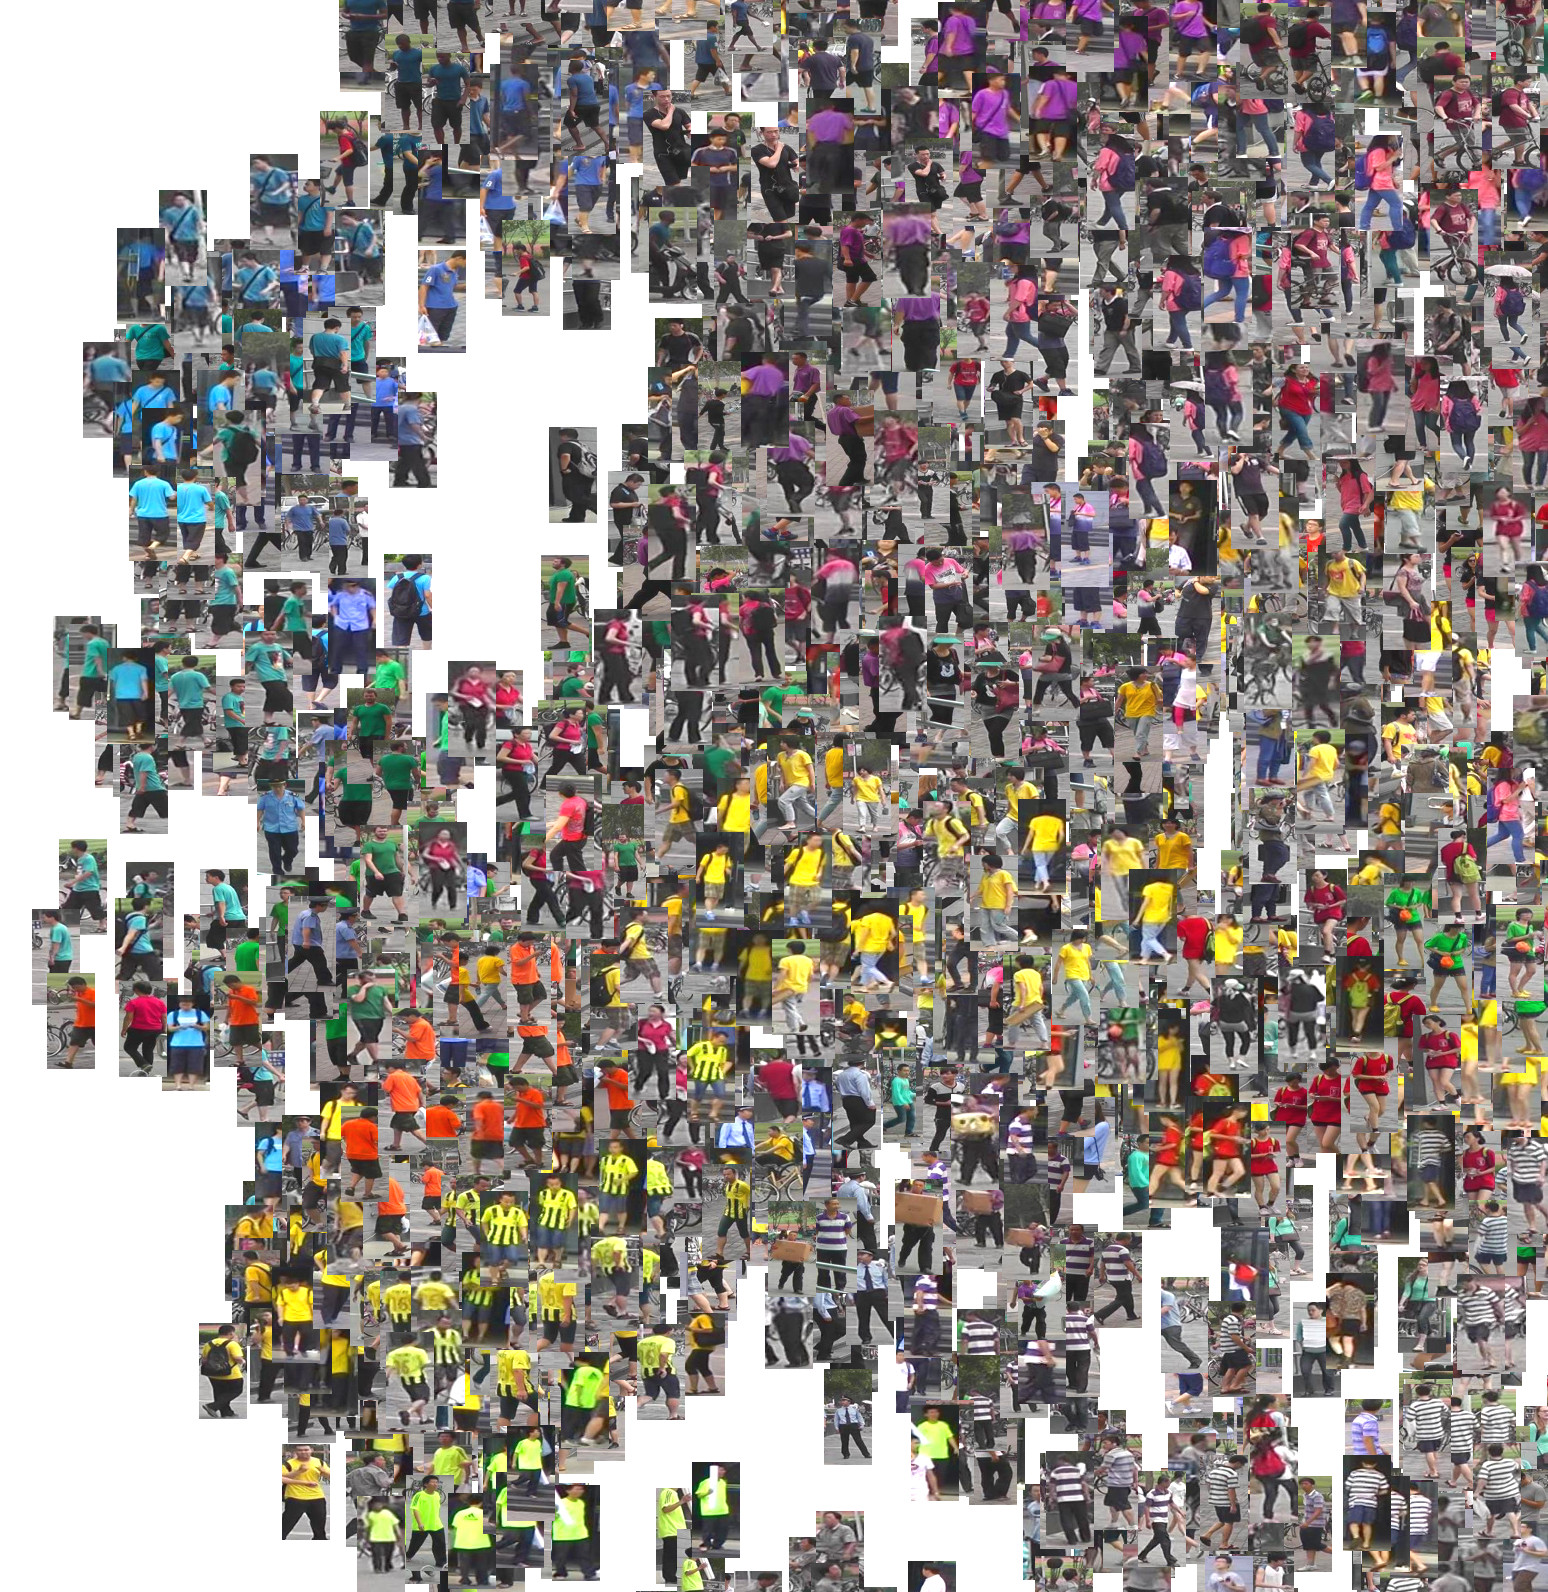
\includegraphics[width=0.6\textwidth]{informatica/embedding_paper_principal}
		\caption{Imagen extraída de \cite{informatica:principal}}
	\end{figure}

\end{frame}

\begin{frame}{Redes siamesas}

	\begin{figure}
		\includegraphics[width=0.9\textwidth]{informatica/siamesa_firma}
		\caption{Imagen extraída de \cite{informatica:siamesa_web_imagen}.}
		\label{img:siamesa_firma}
	\end{figure}

	\begin{itemize}
		\item Herramienta para aprender el \textit{embedding}.
		\item Se utiliza o \textit{contrastive loss} (pares) o \textit{triplet loss} (triples).
	\end{itemize}

\end{frame}

\begin{frame}{Triplet Loss}
	\begin{figure}
		\includegraphics[width=1.0\textwidth]{informatica/triplet_loss_learning}
		\caption{Imágenes extraídas de \cite{informatica:cacd_dataset}.}
	\end{figure}

	A partir de:
	\begin{equation}
		D_{A, P} \leq D_{A, N},
	\end{equation}

	llegamos a:

	\begin{equation} \label{ieq:triplet_loss_single_entry}
		\mathcal{L}_{tri}(\theta; A, P, N) := max \{D_{A, P} - D_{A, N} + \alpha, 0 \}
	\end{equation}
\end{frame}

\begin{frame}{Variantes \textit{online} sobre \textit{Triplet Loss}}

	\begin{itemize}
		\item Problema: necesitamos generar los triples de forma \textit{offline}.
		\item Solución: generar los \textit{batches} de forma \textit{online}.
		      \begin{itemize}
			      \item Usando \textit{P-K} sampling.
			      \item Aplicando las variantes \textit{Batch All} y \textit{Batch Hard} sobre estos nuevos \textit{batches}
		      \end{itemize}
	\end{itemize}

\end{frame}

\begin{frame}{\textit{P-K} sampling}

	\begin{figure}
		\includegraphics[width=0.6\textwidth]{informatica/ejemplo_grafico_pk_sampling}
		\caption{Imagen extraída de \cite{informatica:paper_image_pk_sampling}.}
	\end{figure}

	\begin{itemize}
		\item Elegimos $P$ clases aleatorias.
		\item Por cada clase, elegimos $K$ imágenes aleatorias.
	\end{itemize}

\end{frame}

\begin{frame}{Variantes \textit{online}}

	Sobre el anterior \textit{P-K} sampling:

	\begin{itemize}
		\item \textit{Batch All}: probar todas las combinaciones ancla - positivo - negativo.
		\item \textit{Batch Hard}: por cada ancla, computar la pérdida con el positivo más lejano y el negativo más cercano (combinación más complicada).
	\end{itemize}

\end{frame}

\subsection{Experimentación preliminar}
\begin{frame}{Resultados preliminares sobre \textit{CACD}}

\end{frame}

\begin{frame}{Resultados preliminares sobre \textit{MNIST}}

\end{frame}
